% RESULTS gallery (P1 analog: p1_fig9). AUTO-GENERATED by no_upload/gen_results_gallery_p3.py.
% Tiles are real results/leaderboard/metric plots cropped from each benchmark's arXiv paper;
% provenance in Table~\ref{tab:results_provenance}. Grouped by type of evidence.
\begin{figure*}[p]
\centering
\definecolor{rgA}{HTML}{1F618D}\definecolor{rgB}{HTML}{117A65}\definecolor{rgC}{HTML}{B9770E}%
\resizebox{\textwidth}{!}{%
\begin{tikzpicture}[x=1cm,y=1cm]
\fill[black!88] (0,0) rectangle (13.62,-0.72);
\node[anchor=west,text=white,font=\large\bfseries,inner sep=0] at (0.16,-0.36) {Results reported across the surveyed corpus};
\node[anchor=east,text=white!70,font=\scriptsize,inner sep=0] at (13.46,-0.36) {vector, zoomable, per-panel arXiv links};
\fill[rgA!82!black] (0,-0.720) rectangle (13.62,-1.220);
\node[anchor=west,text=white,font=\footnotesize\bfseries,inner sep=0] at (0.12,-0.970) {Leaderboard \& model-comparison charts};
\node[anchor=north west,inner sep=0] at (0.060,-1.290) {\href{https://arxiv.org/abs/2510.18135}{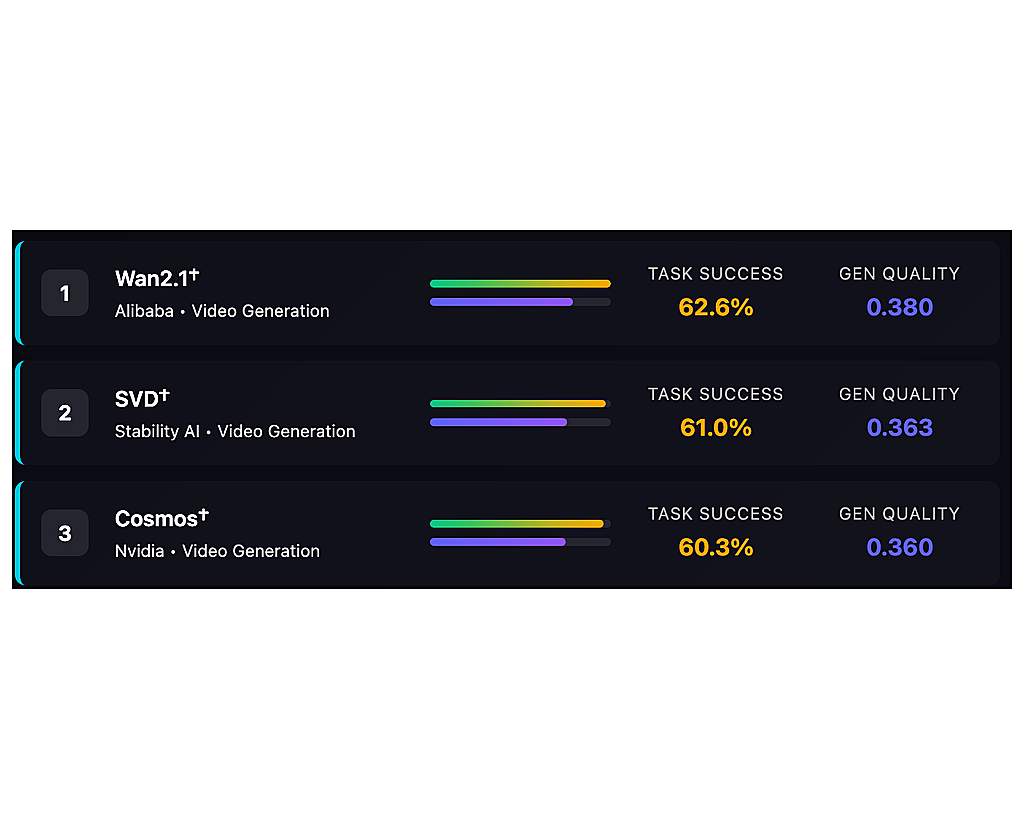
\includegraphics[width=3.300cm,height=2.640cm]{figures/img/results_tiles/worldinworld.png}}};
\draw[black!35,line width=0.35pt] (0.060,-1.290) rectangle (3.360,-3.930);
\node[anchor=north west,text=ACMDarkBlue,font=\scriptsize,inner sep=0] at (0.080,-3.950) {\href{https://arxiv.org/abs/2510.18135}{World-in-World}};
\node[anchor=north west,text=black!55,font=\tiny,inner sep=0] at (0.080,-4.180) {\href{https://arxiv.org/abs/2510.18135}{arXiv:2510.18135}};
\node[anchor=north west,inner sep=0] at (3.420,-1.290) {\href{https://arxiv.org/abs/2310.11440}{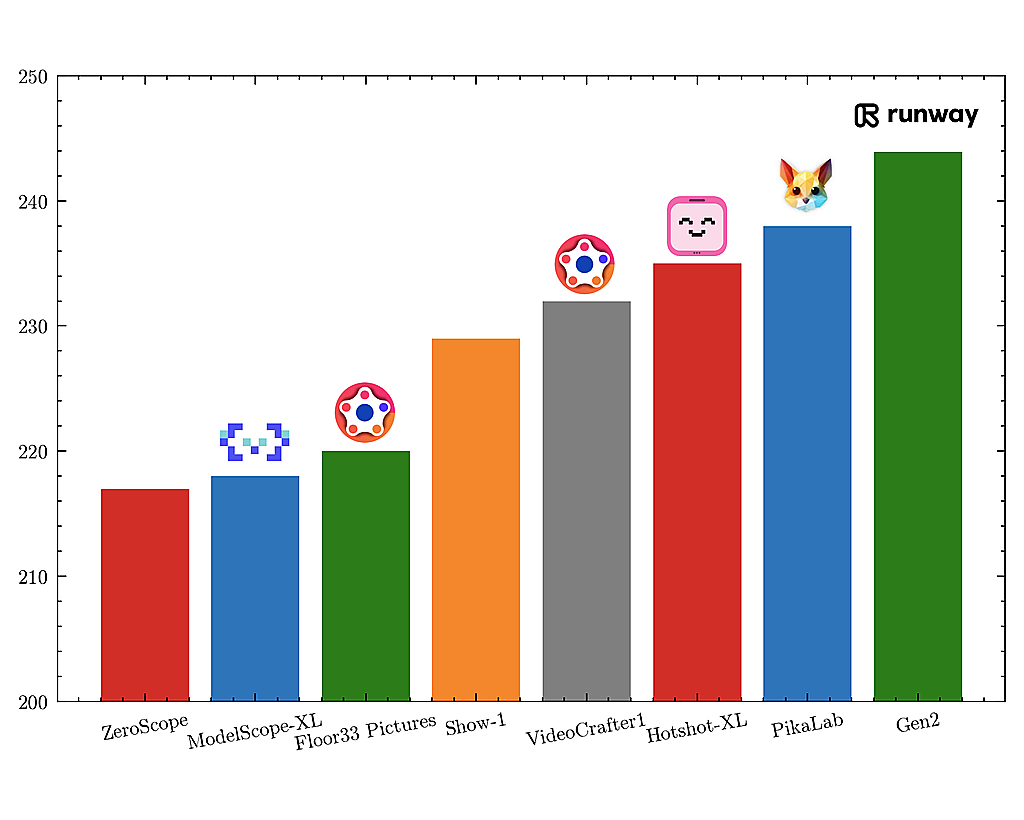
\includegraphics[width=3.300cm,height=2.640cm]{figures/img/results_tiles/evalcrafter_bars.png}}};
\draw[black!35,line width=0.35pt] (3.420,-1.290) rectangle (6.720,-3.930);
\node[anchor=north west,text=ACMDarkBlue,font=\scriptsize,inner sep=0] at (3.440,-3.950) {\href{https://arxiv.org/abs/2310.11440}{EvalCrafter}};
\node[anchor=north west,text=black!55,font=\tiny,inner sep=0] at (3.440,-4.180) {\href{https://arxiv.org/abs/2310.11440}{arXiv:2310.11440}};
\node[anchor=north west,inner sep=0] at (6.780,-1.290) {\href{https://arxiv.org/abs/2406.15252}{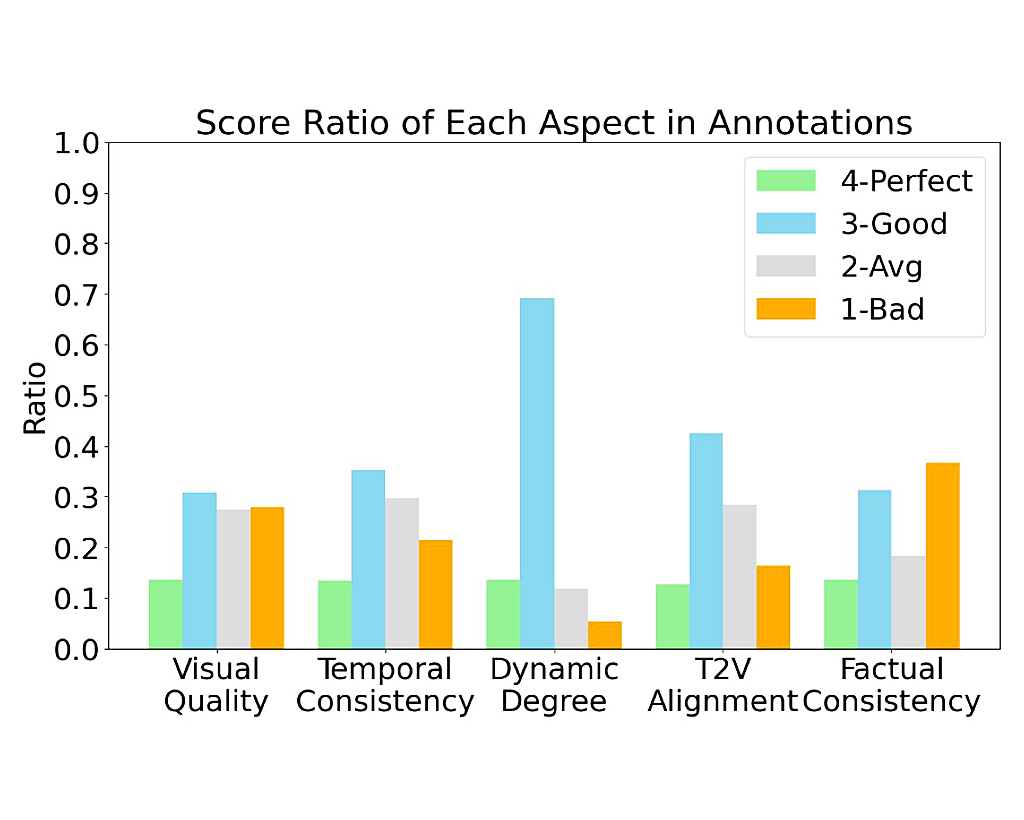
\includegraphics[width=3.300cm,height=2.640cm]{figures/img/results_tiles/videoscore.png}}};
\draw[black!35,line width=0.35pt] (6.780,-1.290) rectangle (10.080,-3.930);
\node[anchor=north west,text=ACMDarkBlue,font=\scriptsize,inner sep=0] at (6.800,-3.950) {\href{https://arxiv.org/abs/2406.15252}{VideoScore}};
\node[anchor=north west,text=black!55,font=\tiny,inner sep=0] at (6.800,-4.180) {\href{https://arxiv.org/abs/2406.15252}{arXiv:2406.15252}};
\node[anchor=north west,inner sep=0] at (10.140,-1.290) {\href{https://arxiv.org/abs/2502.20694}{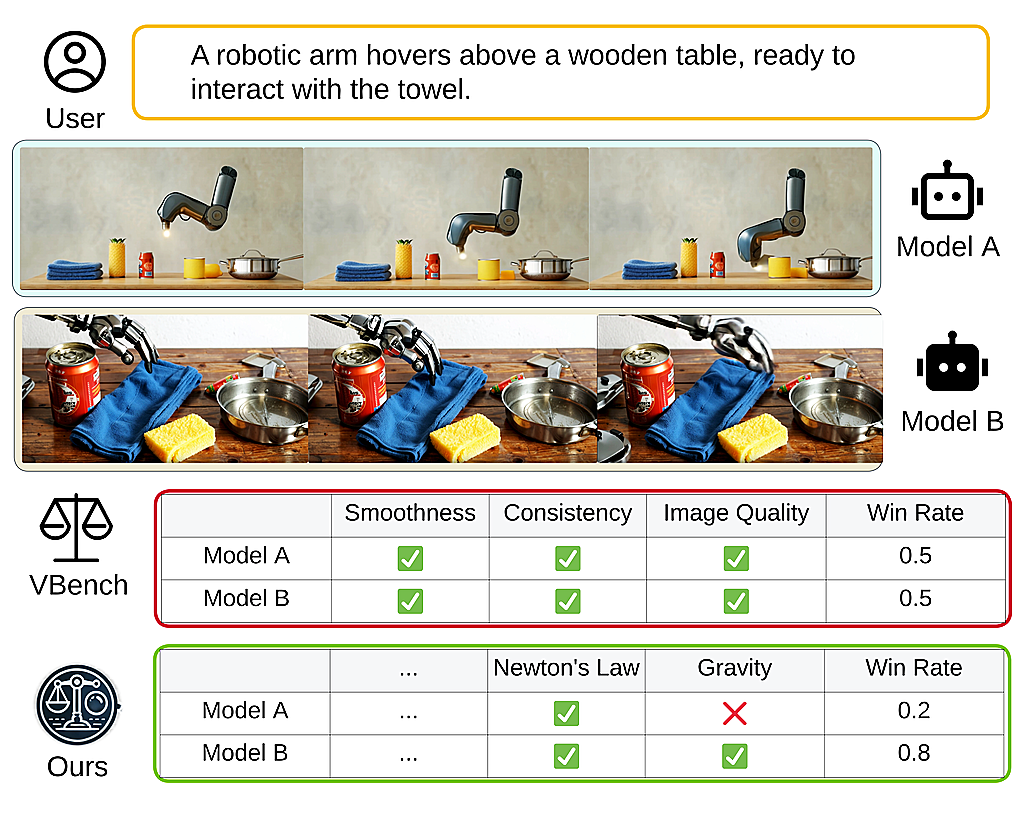
\includegraphics[width=3.300cm,height=2.640cm]{figures/img/results_tiles/worldmodelbench.png}}};
\draw[black!35,line width=0.35pt] (10.140,-1.290) rectangle (13.440,-3.930);
\node[anchor=north west,text=ACMDarkBlue,font=\scriptsize,inner sep=0] at (10.160,-3.950) {\href{https://arxiv.org/abs/2502.20694}{WorldModelBench}};
\node[anchor=north west,text=black!55,font=\tiny,inner sep=0] at (10.160,-4.180) {\href{https://arxiv.org/abs/2502.20694}{arXiv:2502.20694}};
\fill[rgB!82!black] (0,-4.690) rectangle (13.62,-5.190);
\node[anchor=west,text=white,font=\footnotesize\bfseries,inner sep=0] at (0.12,-4.940) {Per-dimension radar \& multi-metric};
\node[anchor=north west,inner sep=0] at (0.060,-5.260) {\href{https://arxiv.org/abs/2311.17982}{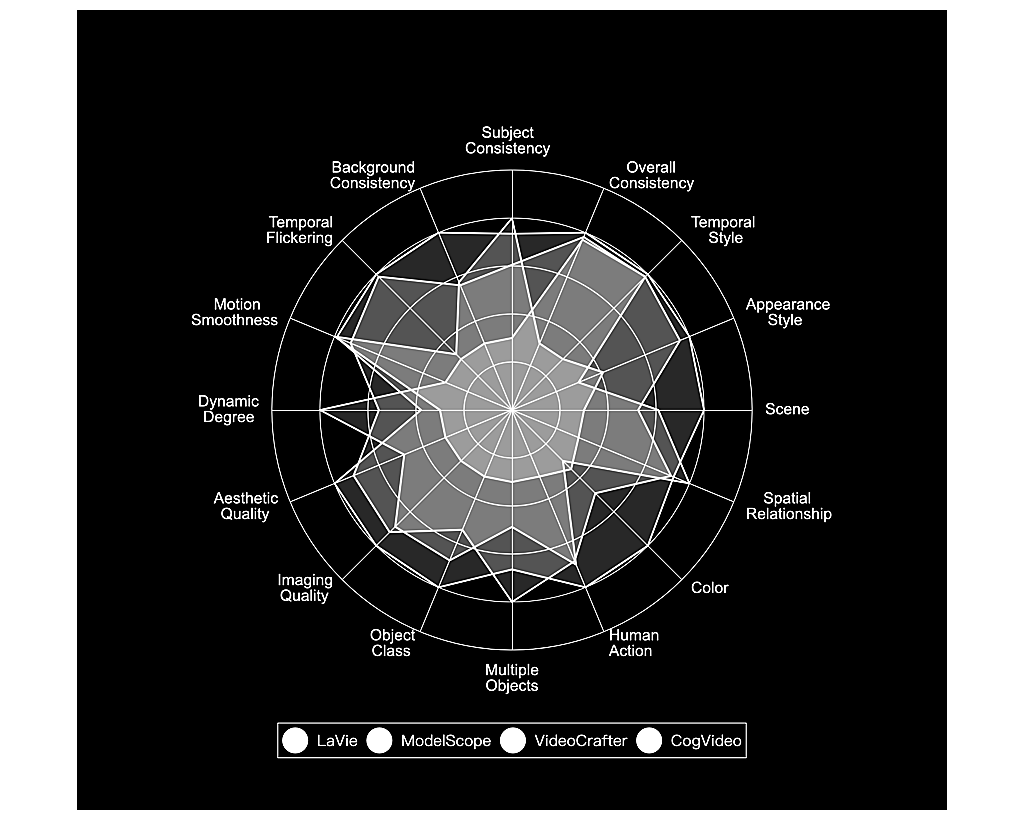
\includegraphics[width=3.300cm,height=2.640cm]{figures/img/results_tiles/vbench_radar.png}}};
\draw[black!35,line width=0.35pt] (0.060,-5.260) rectangle (3.360,-7.900);
\node[anchor=north west,text=ACMDarkBlue,font=\scriptsize,inner sep=0] at (0.080,-7.920) {\href{https://arxiv.org/abs/2311.17982}{VBench}};
\node[anchor=north west,text=black!55,font=\tiny,inner sep=0] at (0.080,-8.150) {\href{https://arxiv.org/abs/2311.17982}{arXiv:2311.17982}};
\node[anchor=north west,inner sep=0] at (3.420,-5.260) {\href{https://arxiv.org/abs/2505.09694}{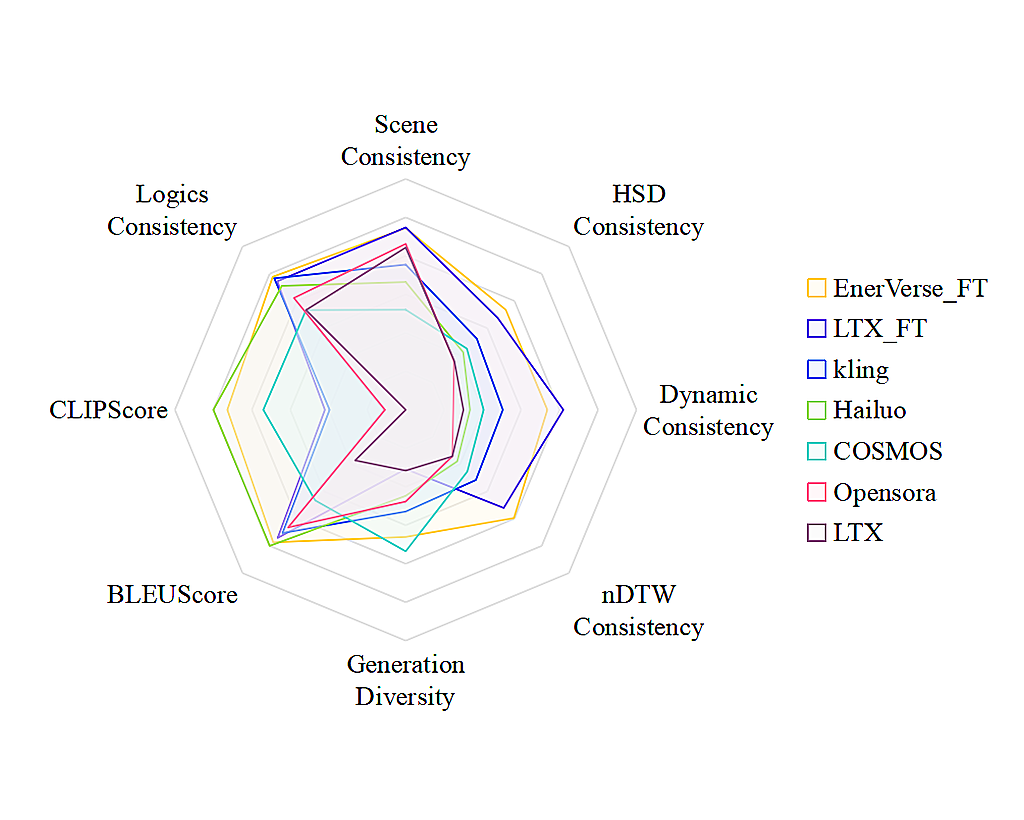
\includegraphics[width=3.300cm,height=2.640cm]{figures/img/results_tiles/ewmbench.png}}};
\draw[black!35,line width=0.35pt] (3.420,-5.260) rectangle (6.720,-7.900);
\node[anchor=north west,text=ACMDarkBlue,font=\scriptsize,inner sep=0] at (3.440,-7.920) {\href{https://arxiv.org/abs/2505.09694}{EWMBench}};
\node[anchor=north west,text=black!55,font=\tiny,inner sep=0] at (3.440,-8.150) {\href{https://arxiv.org/abs/2505.09694}{arXiv:2505.09694}};
\node[anchor=north west,inner sep=0] at (6.780,-5.260) {\href{https://arxiv.org/abs/2602.08971}{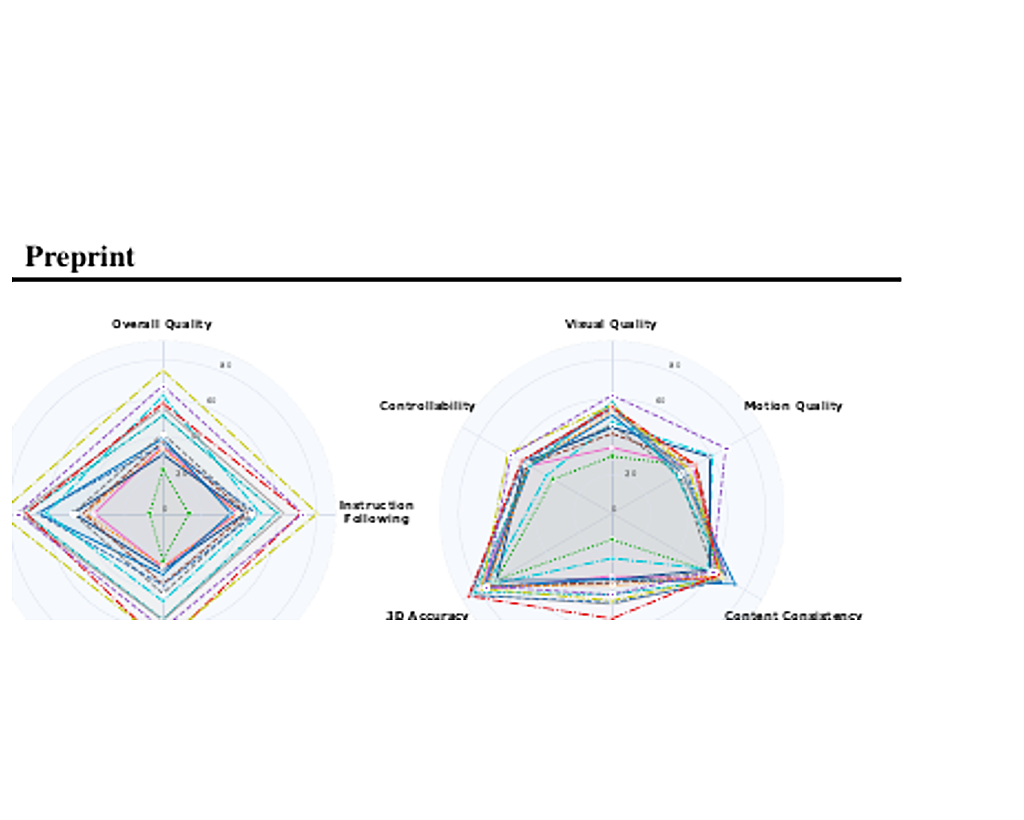
\includegraphics[width=3.300cm,height=2.640cm]{figures/img/results_tiles/worldarena.png}}};
\draw[black!35,line width=0.35pt] (6.780,-5.260) rectangle (10.080,-7.900);
\node[anchor=north west,text=ACMDarkBlue,font=\scriptsize,inner sep=0] at (6.800,-7.920) {\href{https://arxiv.org/abs/2602.08971}{WorldArena}};
\node[anchor=north west,text=black!55,font=\tiny,inner sep=0] at (6.800,-8.150) {\href{https://arxiv.org/abs/2602.08971}{arXiv:2602.08971}};
\node[anchor=north west,inner sep=0] at (10.140,-5.260) {\href{https://arxiv.org/abs/2310.11440}{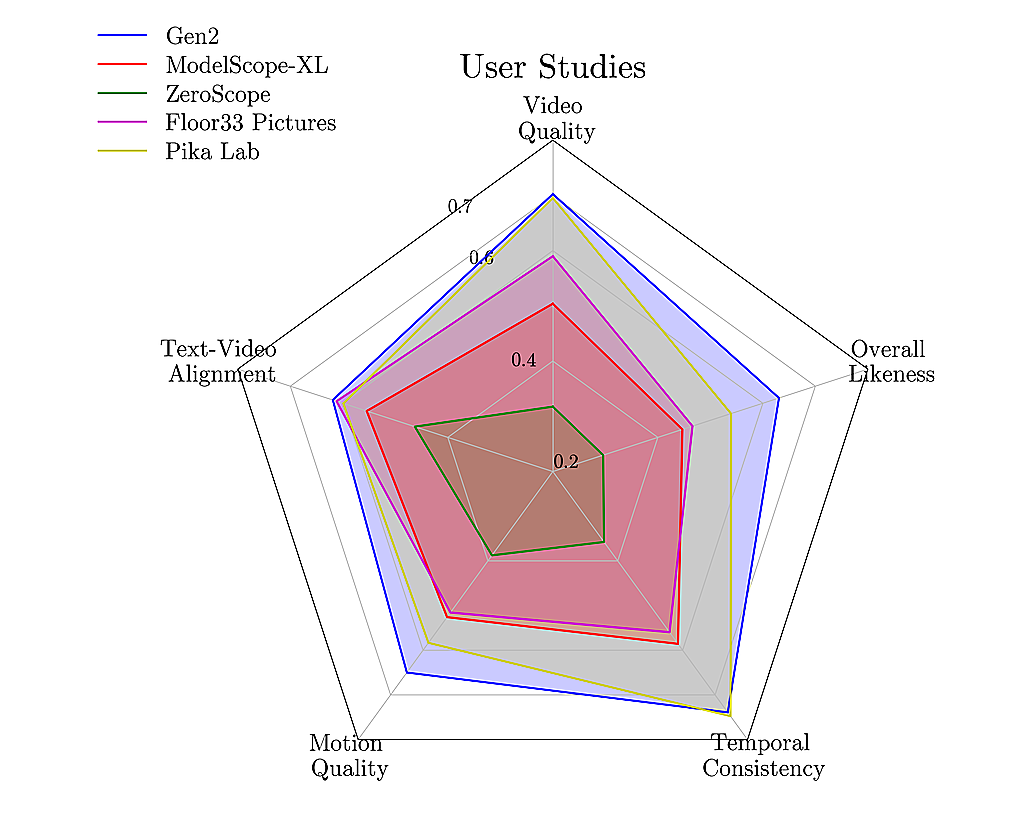
\includegraphics[width=3.300cm,height=2.640cm]{figures/img/results_tiles/evalcrafter_userradar.png}}};
\draw[black!35,line width=0.35pt] (10.140,-5.260) rectangle (13.440,-7.900);
\node[anchor=north west,text=ACMDarkBlue,font=\scriptsize,inner sep=0] at (10.160,-7.920) {\href{https://arxiv.org/abs/2310.11440}{EvalCrafter}};
\node[anchor=north west,text=black!55,font=\tiny,inner sep=0] at (10.160,-8.150) {\href{https://arxiv.org/abs/2310.11440}{arXiv:2310.11440}};
\fill[rgC!82!black] (0,-8.660) rectangle (13.62,-9.160);
\node[anchor=west,text=white,font=\footnotesize\bfseries,inner sep=0] at (0.12,-8.910) {Distributions \& composition};
\node[anchor=north west,inner sep=0] at (0.060,-9.230) {\href{https://arxiv.org/abs/2310.11440}{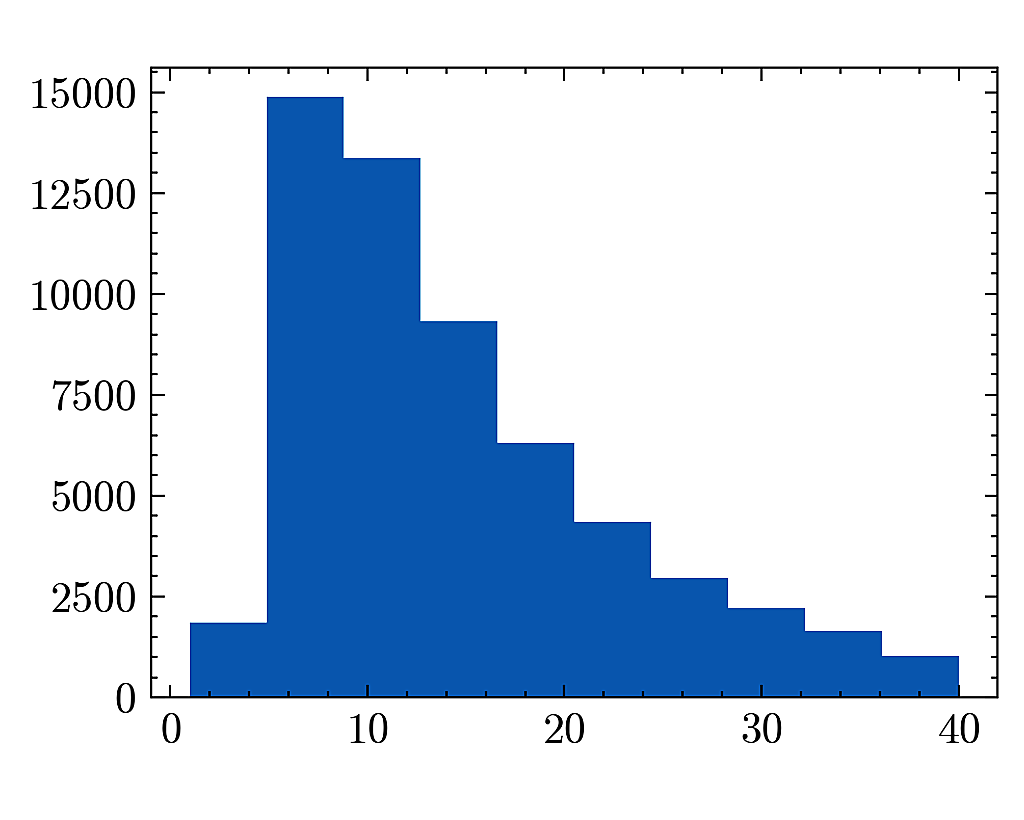
\includegraphics[width=3.300cm,height=2.640cm]{figures/img/results_tiles/evalcrafter_hist.png}}};
\draw[black!35,line width=0.35pt] (0.060,-9.230) rectangle (3.360,-11.870);
\node[anchor=north west,text=ACMDarkBlue,font=\scriptsize,inner sep=0] at (0.080,-11.890) {\href{https://arxiv.org/abs/2310.11440}{EvalCrafter}};
\node[anchor=north west,text=black!55,font=\tiny,inner sep=0] at (0.080,-12.120) {\href{https://arxiv.org/abs/2310.11440}{arXiv:2310.11440}};
\node[anchor=north west,inner sep=0] at (3.420,-9.230) {\href{https://arxiv.org/abs/2310.11440}{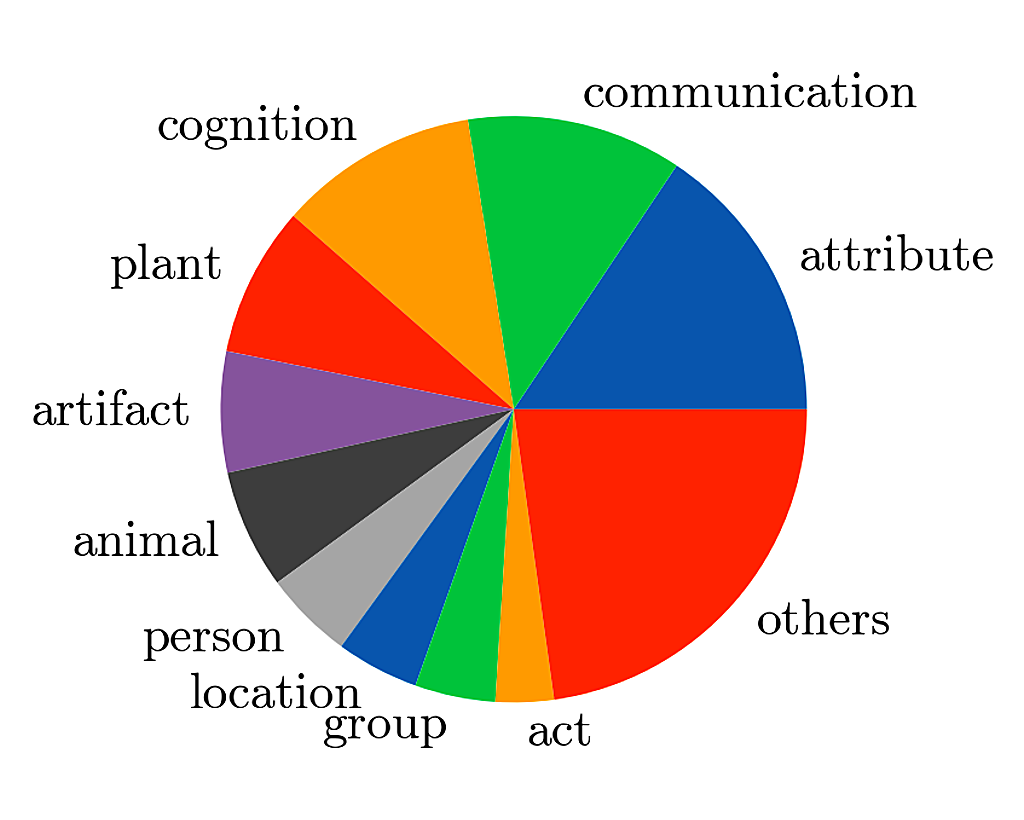
\includegraphics[width=3.300cm,height=2.640cm]{figures/img/results_tiles/evalcrafter_pie.png}}};
\draw[black!35,line width=0.35pt] (3.420,-9.230) rectangle (6.720,-11.870);
\node[anchor=north west,text=ACMDarkBlue,font=\scriptsize,inner sep=0] at (3.440,-11.890) {\href{https://arxiv.org/abs/2310.11440}{EvalCrafter}};
\node[anchor=north west,text=black!55,font=\tiny,inner sep=0] at (3.440,-12.120) {\href{https://arxiv.org/abs/2310.11440}{arXiv:2310.11440}};
\node[anchor=north west,inner sep=0] at (6.780,-9.230) {\href{https://arxiv.org/abs/2311.17982}{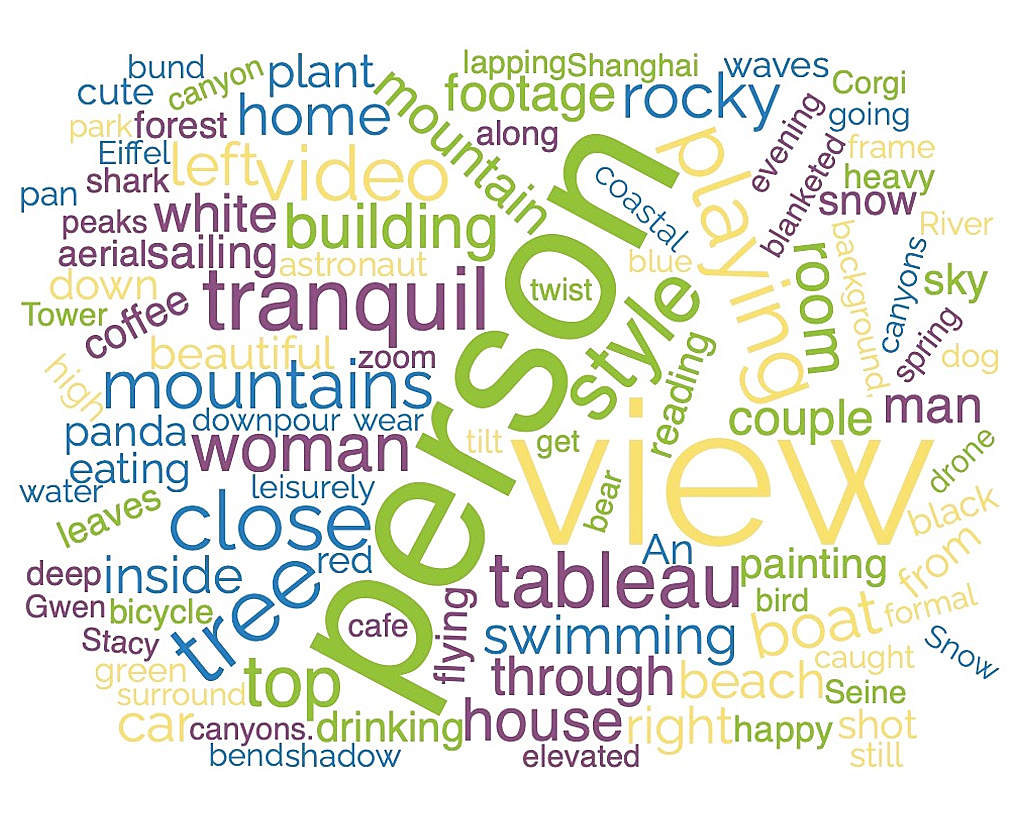
\includegraphics[width=3.300cm,height=2.640cm]{figures/img/results_tiles/vbench_wordcloud.png}}};
\draw[black!35,line width=0.35pt] (6.780,-9.230) rectangle (10.080,-11.870);
\node[anchor=north west,text=ACMDarkBlue,font=\scriptsize,inner sep=0] at (6.800,-11.890) {\href{https://arxiv.org/abs/2311.17982}{VBench}};
\node[anchor=north west,text=black!55,font=\tiny,inner sep=0] at (6.800,-12.120) {\href{https://arxiv.org/abs/2311.17982}{arXiv:2311.17982}};
\node[anchor=north west,inner sep=0] at (10.140,-9.230) {\href{https://arxiv.org/abs/2406.03520}{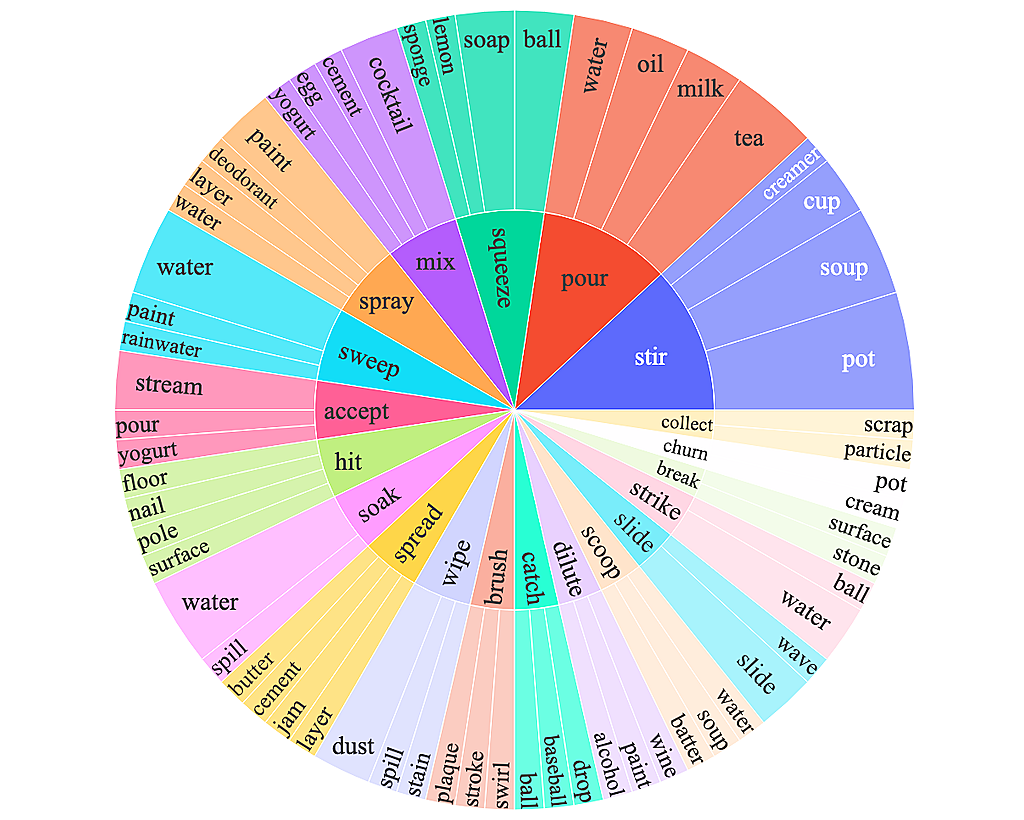
\includegraphics[width=3.300cm,height=2.640cm]{figures/img/results_tiles/videophy_sunburst.png}}};
\draw[black!35,line width=0.35pt] (10.140,-9.230) rectangle (13.440,-11.870);
\node[anchor=north west,text=ACMDarkBlue,font=\scriptsize,inner sep=0] at (10.160,-11.890) {\href{https://arxiv.org/abs/2406.03520}{VideoPhy}};
\node[anchor=north west,text=black!55,font=\tiny,inner sep=0] at (10.160,-12.120) {\href{https://arxiv.org/abs/2406.03520}{arXiv:2406.03520}};
\end{tikzpicture}}
\caption{\textbf{Results reported across the surveyed corpus.} Representative results figures from the catalogue, grouped by type of evidence: \emph{leaderboard and model-comparison charts}, \emph{per-dimension radar and multi-metric} plots, and \emph{distributions and composition}. Each panel is a live hyperlink to the source paper on arXiv and is annotated with its arXiv id (per-panel provenance in Table~\ref{tab:results_provenance}); the figure is vector with plots embedded at full resolution. Only results/leaderboard/metric figures are shown; task and scene figures appear in Figure~\ref{fig:subject_gallery}. As a benchmark survey the reported evidence is dominated by rankings, radars and distributions rather than training curves, and is sparser than the subject figures, so this gallery is smaller; benchmarks that publish no results figure are omitted, not fabricated. A benchmark may appear more than once when it reports several evidence types. Images \textcopyright\ their respective authors, reproduced for scholarly review.}
\Description{A gallery of benchmark results figures in three evidence-type bands. The top band, leaderboard and model-comparison charts, shows four ranking bar charts and win-rate tables. The middle band, per-dimension radar and multi-metric, shows three radar plots over evaluation dimensions. The bottom band, distributions and composition, shows a prompt-length histogram, a meta-type pie chart, and a prompt word cloud. Each panel is labelled with the benchmark name and its arXiv id.}
\label{fig:results_gallery}
\end{figure*}
